% -------------------------------------------------------
\section{Эксперимент 3: Задача открытия правила 2-4-6}
% -------------------------------------------------------

\subsection{Обоснование выбора парадигмы}

Задача открытия правила 2-4-6, введённая Уэйсоном~\cite{wason1960failure}, является классической парадигмой для исследования предубеждения подтверждения в индуктивном рассуждении. В оригинальном эксперименте испытуемым сообщалось, что тройка $(2, 4, 6)$ удовлетворяет скрытому правилу, и предлагалось открыть его, предлагая новые тройки и получая бинарную обратную связь. Канонический результат: испытуемые тестируют тройки, согласующиеся с текущей гипотезой (например, $(4, 8, 10)$ для гипотезы «чётные числа в порядке возрастания»), вместо попыток фальсифицировать её, и не обнаруживают истинное правило («любая возрастающая последовательность»).

В отличие от экспериментов 1 и 2, где предубеждение проявляется в единственном ответе, здесь оно измеряется как свойство \textit{стратегии} на протяжении многоходового диалога.

\subsection{Конструкция датасета правил: пять таксономических категорий}

Был сформирован независимый датасет из \textbf{50 правил}, организованных в пять таксономических категорий:

\begin{itemize}
  \item \textbf{Порядок и сравнение} (9 правил) --- отношения между элементами: $x < y < z$, $x > y \land z > y$;
  \item \textbf{Чётность и делимость} (10 правил) --- свойства модульной арифметики: все чётные, сумма кратна 3;
  \item \textbf{Арифметические отношения} (10 правил) --- аддитивные и мультипликативные структуры: $x + y = z$, $y - x = z - y$;
  \item \textbf{Структурные паттерны} (11 правил) --- позиционные и теоретико-множественные свойства: $\max(x, y, z) = z$, ровно два уникальных значения;
  \item \textbf{Смешанные / составные} (10 правил) --- конъюнкции из предыдущих категорий: $x < y < z \land (x + y + z) \equiv 0 \pmod{2}$.
\end{itemize}

Все правила верифицированы на исполнимость в диапазоне $[1, 99]^3$, отсутствие функциональных дубликатов (проверка через экстенсиональную эквивалентность) и отсутствие тавтологий. Ряд правил намеренно сконструирован как \textit{ловушки специфичности}: правила, являющиеся строго более специфичными, чем истинное правило, но согласующиеся с порождающей тройкой $(2, 4, 6)$. Из 50 правил \textbf{26 удовлетворяются} тройкой $(2, 4, 6)$ и 24 не удовлетворяются.

\subsection{Многоходовой диалоговый протокол}

Эксперимент реализован как многоходовой диалог. На каждом ходу $t$ модель получает историю разговора и должна ответить в строго ограниченном формате:

\begin{quote}
\texttt{H: lambda x, y, z: <hypothesis>}\\
\texttt{T: [x, y, z]}
\end{quote}

где \texttt{H} --- исполняемый Python-лямбда-выражение, представляющее текущую гипотезу о скрытом правиле $R$, а \texttt{T} --- следующая тройка для тестирования. Модель получает только бинарную обратную связь вида \texttt{(a, b, c) -> True} или \texttt{(a, b, c) -> False}. Испытание завершается либо по достижении \texttt{max\_turns}, либо при выполнении условия ранней остановки: $\text{IOU}(H_t, R) > 0{,}95$ на текущей Монте-Карло выборке~--- в зависимости от того, что наступит раньше. Это объясняет, почему среднее число ходов у reasoning-модели (\texttt{mean\_turns} $\approx 15$) меньше \texttt{max\_turns}: часть траекторий завершается досрочно при успешном обнаружении правила. В отличие от бенчмарка WILT~\cite{banatt2024wilt}, дизайн настоящего исследования требует от модели поддерживать живую, исполняемую гипотезу \textit{на каждом ходу}, что позволяет анализировать полную траекторию гипотез.

\subsection{Промпт-условия: Baseline и Adaptive}

Оба условия используют одинаковую структуру диалога: стартовое сообщение пользователя содержит только \texttt{True} (подтверждение того, что тройка $(2, 4, 6)$ удовлетворяет правилу), на каждом последующем ходу модель получает бинарную обратную связь вида \texttt{(x, y, z) -> True} или \texttt{(x, y, z) -> False}. Ответ модели должен быть оформлен в блоке \texttt{```python```} и содержать ровно две строки: гипотезу \texttt{H} и тестируемую тройку \texttt{T}.

\textbf{Baseline.} Системный промпт содержит фрейм задачи, требуемый формат и жёсткие технические ограничения без каких-либо метакогнитивных советов:

\begin{quote}
\textit{You have a hidden rule for number triples (x,y,z). The triple (2,4,6) satisfies this rule. Your goal: discover the rule through testing. YOU MUST respond in a fenced python block on EVERY turn [...] Use ONLY positive integers from 1 to 1000 [...] NO explanations, commentary, or reasoning in your response. NO stopping until maximum turns reached.}
\end{quote}

\textbf{Adaptive.} Идентичен baseline по техническим ограничениям и формату, однако дополнен блоком явных метакогнитивных указаний по стратегии тестирования:

\begin{quote}
\textit{CRITICAL TESTING APPROACH: If you get a False result, your hypothesis MUST change to exclude that case. If you get an unexpected True, your hypothesis MUST expand to include it. Prefer tests that could prove your current hypothesis wrong, not just confirm it. Repeatedly proposing triples your current hypothesis already expects to be True is weak testing. Use boundary cases and contrastive cases that distinguish your current hypothesis from nearby alternatives. Consider mathematical properties: sums, products, differences, divisibility, remainders.}
\end{quote}

Манипуляция мотивирована данными Batista и Griffiths~\cite{batista2026rational} о том, что явные инструкции по обратной связи модулируют поведение пересмотра гипотез. Оба условия разделяют требование продолжать тестирование до достижения \texttt{max\_turns} вне зависимости от уверенности модели.

\subsection{Метрики качества гипотез}

\textbf{Ключевой методологической особенностью} является использование \textit{экстенсиональной эквивалентности} для оценки гипотез. Вместо текстового сравнения строк гипотезы оцениваются как множества принятых троек над большой случайной выборкой~\cite{banatt2024wilt}. Формально: для скрытого правила $R$ и гипотезы модели $H_t$ на ходу $t$ сэмплируются $N = 200{,}000$ случайных троек $(x, y, z) \in [1, 99]^3$ и вычисляются булевы векторы $\mathbf{r}$ и $\mathbf{h}_t$. Метрика:
\begin{equation}
  \text{IOU}(H_t, R) = \frac{|\mathbf{h}_t \cap \mathbf{r}|}{|\mathbf{h}_t \cup \mathbf{r}|},
  \label{eq:iou}
\end{equation}
испытание считается \textbf{успешным} при $\text{IOU}(H_T, R) > 0{,}95$.

\textbf{Success Rate} ($\uparrow$) --- доля правил, для которых финальная гипотеза достигает $\text{IOU} > 0{,}95$.

\textbf{Mean AUC-IOU} ($\uparrow$) --- площадь под кривой IOU по ходам, усреднённая по всем правилам:
\begin{equation}
  \text{AUC-IOU} = \frac{1}{T} \sum_{t=1}^{T} \text{IOU}(H_t, R).
  \label{eq:auc_iou}
\end{equation}

\textbf{Confirming Test Rate (CTR)} ($\downarrow$) --- доля ходов, на которых предлагаемая тройка $T_t$ предсказывается текущей гипотезой $H_t$ как True:
\begin{equation}
  \text{CTR} = \frac{1}{T} \sum_{t=1}^{T} \mathbf{1}[H_t(T_t) = \text{True}].
  \label{eq:ctr}
\end{equation}
Напрямую операционализирует предубеждение подтверждения: низкий CTR соответствует фальсификационно-ориентированной стратегии.

\textbf{Hypothesis Change Rate (HCR)} ($\uparrow$) --- доля последовательных пар ходов, на которых модель существенно пересматривает гипотезу:
\begin{equation}
  \text{HCR} = \frac{1}{T-1} \sum_{t=2}^{T} \mathbf{1}[\text{IOU}(H_t, H_{t-1}) < 0{,}9].
  \label{eq:hcr}
\end{equation}
Низкий HCR указывает на «залипание» в начальной гипотезе вне зависимости от полученной обратной связи.

\subsection{Результаты и анализ}

Полные результаты по baseline- и adaptive-условиям представлены в таблице~\ref{tab:246_results}.

\begin{table}[h!]
\caption{Результаты эксперимента 3: baseline и adaptive условия}
\label{tab:246_results}
\centering
\begin{tabular}{|l|c|c|c|c|}
\hline
\textbf{Модель} & \textbf{SR base} & \textbf{SR adap} & \textbf{CTR base} & \textbf{CTR adap} \\
\hline
claude-sonnet-4.6  & 0,28 & 0,28 & 0,812 & 0,787 \\
qwen3.5-397b-a17b  & 0,22 & 0,18 & 0,850 & 0,602 \\
qwen3-next-80b     & 0,20 & 0,24 & 0,976 & 0,719 \\
gpt-5.2            & 0,18 & 0,18 & 0,719 & 0,584 \\
grok-4.1-fast      & 0,14 & 0,08 & 0,629 & 0,672 \\
deepseek-v3.2      & 0,10 & 0,16 & 0,879 & 0,768 \\
gemma-3-12b-it     & 0,06 & 0,04 & 0,747 & 0,718 \\
glm-4.7-flash      & 0,04 & 0,06 & 0,739 & 0,486 \\
gemma-3-27b-it     & 0,04 & 0,10 & 0,688 & 0,842 \\
\hline
claude-sonnet-4.6 reasoning & 0,28 & 0,32 & 0,771 & 0,781 \\
gpt-5.2 reasoning  & 0,38 & 0,48 & 0,726 & 0,559 \\
\hline
\end{tabular}
\end{table}

\begin{figure}[ht]
    \centering
    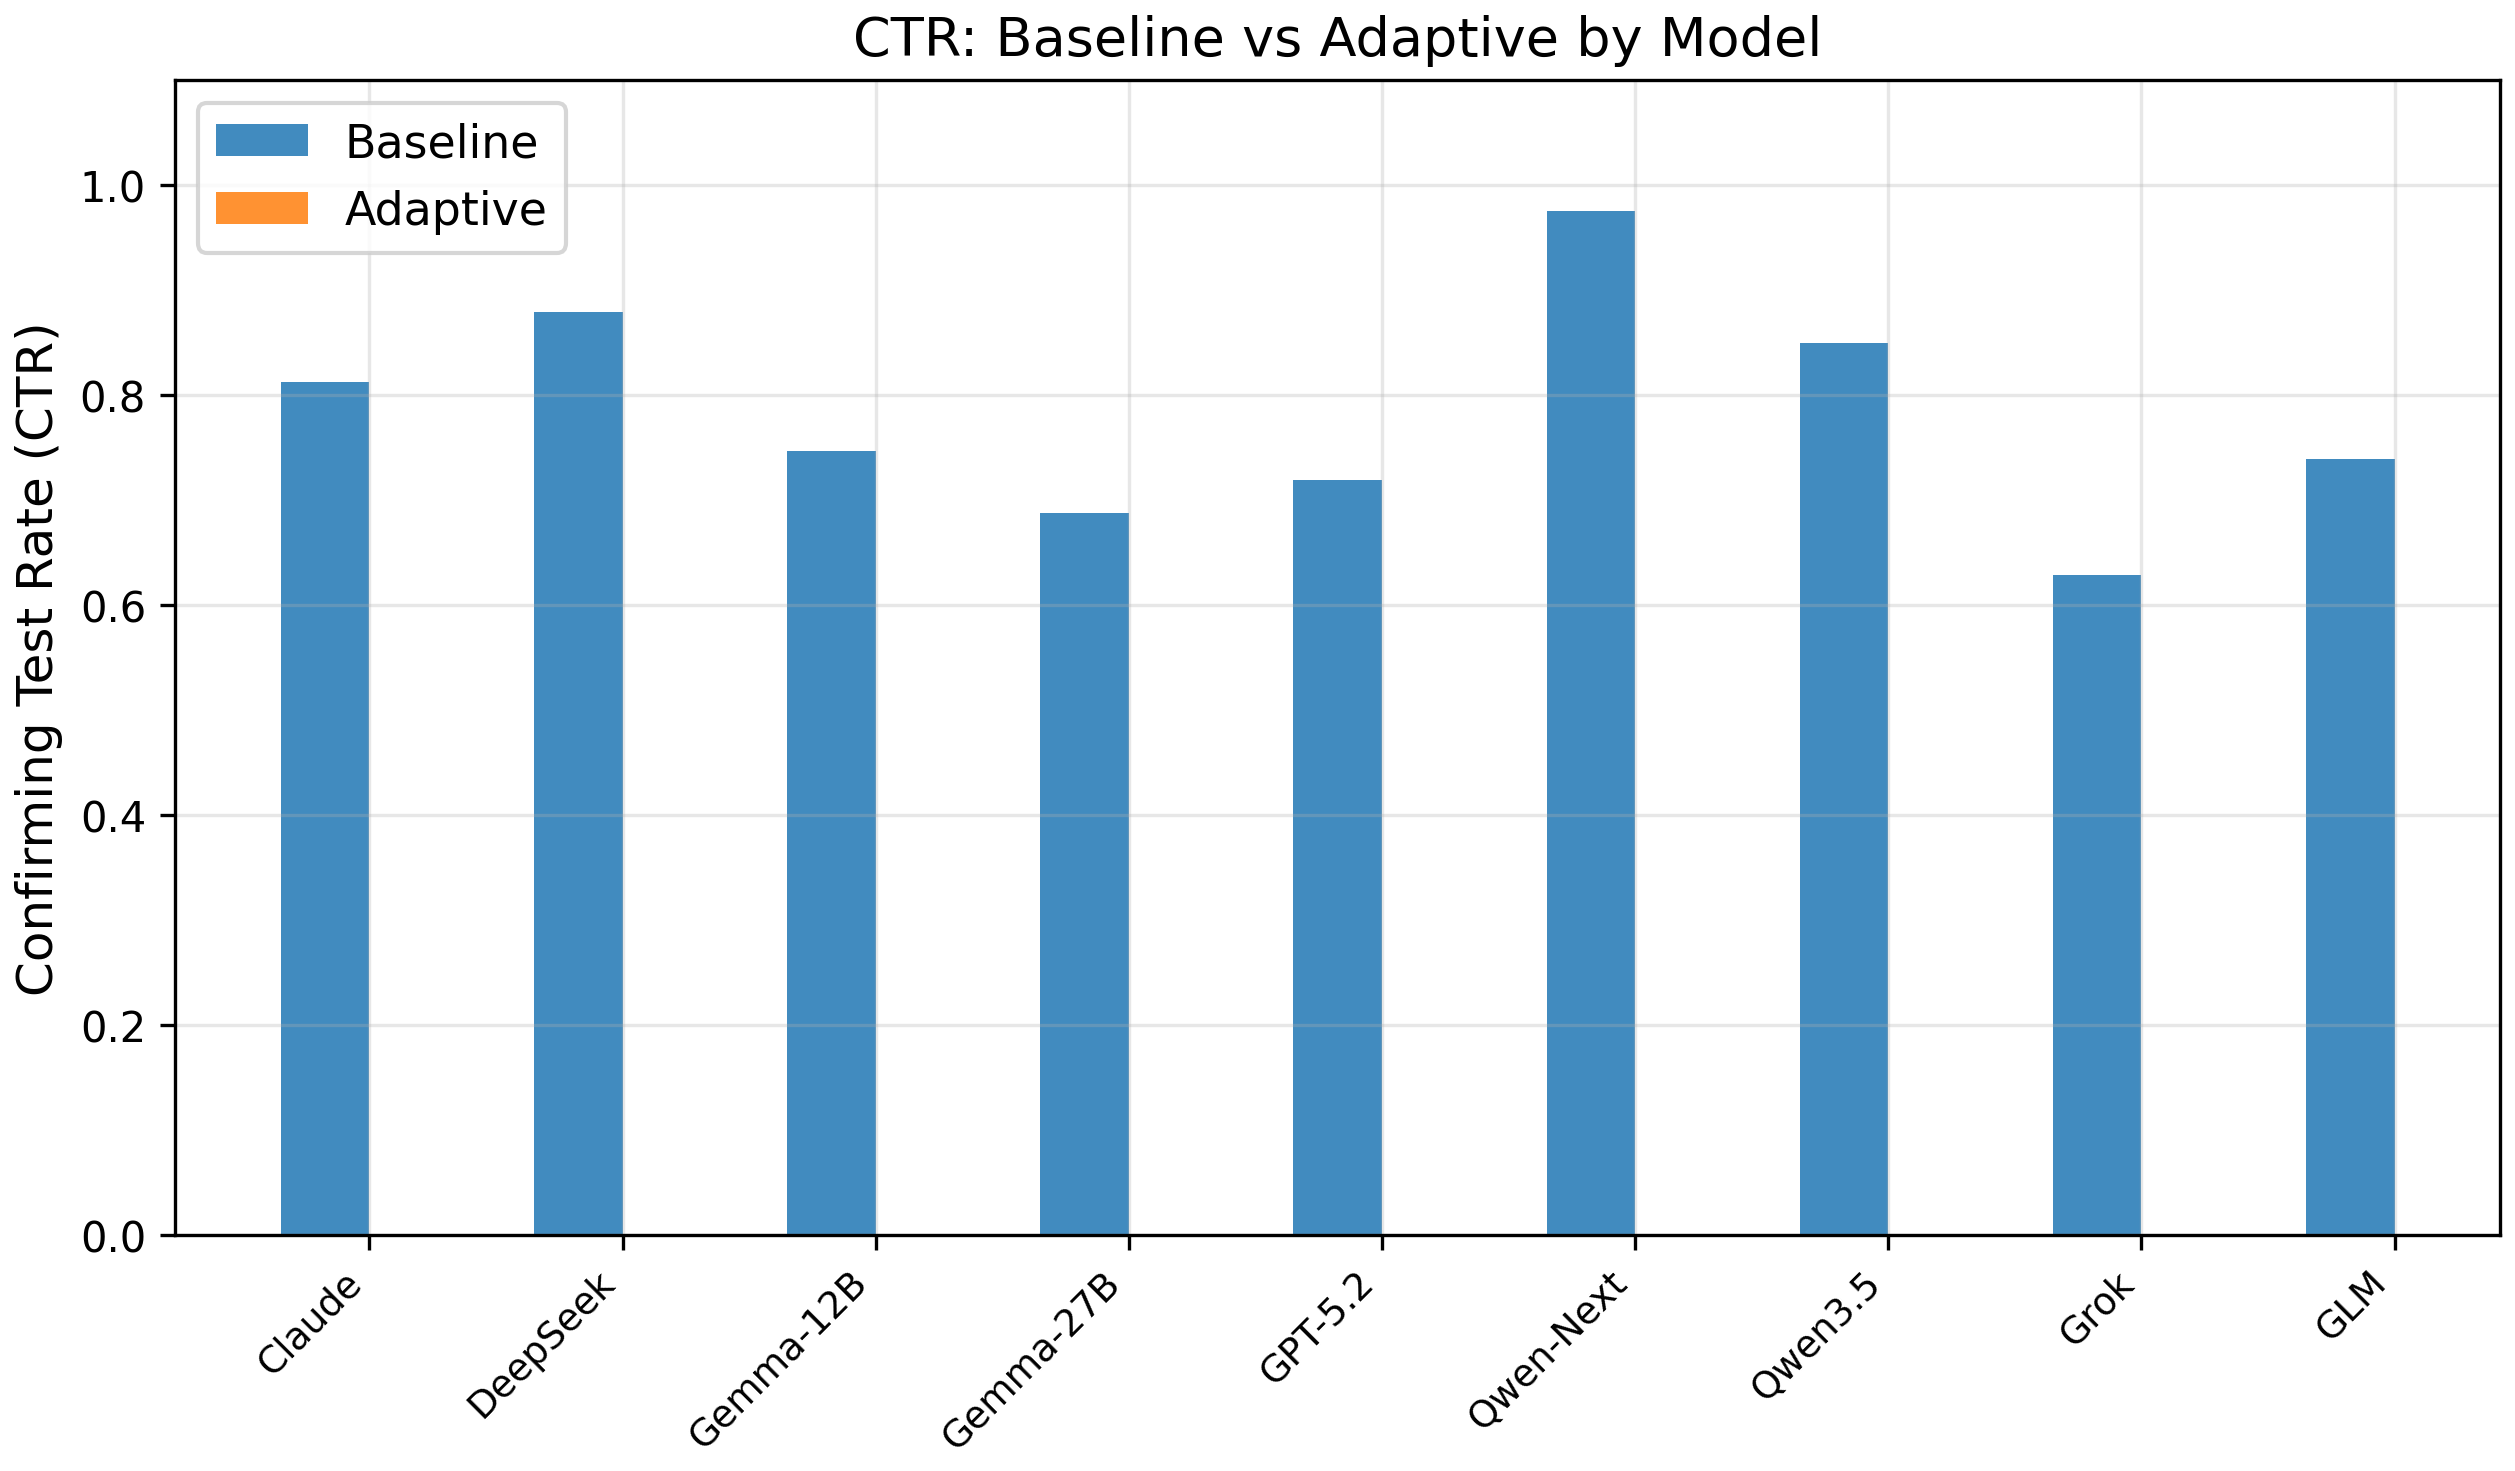
\includegraphics[width=0.8\textwidth]{../experiments_raw_results/wason-2-4-6/figures/wason246_ctr_bars.png}
    \caption{Сравнение коэффициента подтверждающего тестирования (CTR) в условиях Baseline и Adaptive. Снижение CTR в Adaptive указывает на переход к более фальсификационной стратегии.}
    \label{fig:246_ctr_bars}
\end{figure}

\textbf{Гипотеза H1 подтверждена полностью:} CTR в baseline-условии варьируется от 0,629 у \texttt{grok-4.1-fast} до 0,976 у \texttt{qwen3-next-80b} (рис.~\ref{fig:246_ctr_bars}). Даже наименее «подтверждающая» модель в 63\% случаев тестирует тройки, которые её же текущая гипотеза предсказывает как True. Нормативная стратегия байесовского агента предполагает CTR близкий к нулю.

\textbf{Success Rate низкий у всех non-reasoning моделей.} Лучший результат в baseline среди них --- \texttt{claude-sonnet-4.6} с SR $= 0{,}28$, что означает успешное открытие правила лишь в 14 из 50 случаев. \texttt{gemma-3-27b-it} и \texttt{glm-4.7-flash} открывают правило лишь в двух случаях из 50.

\begin{figure}[ht]
    \centering
    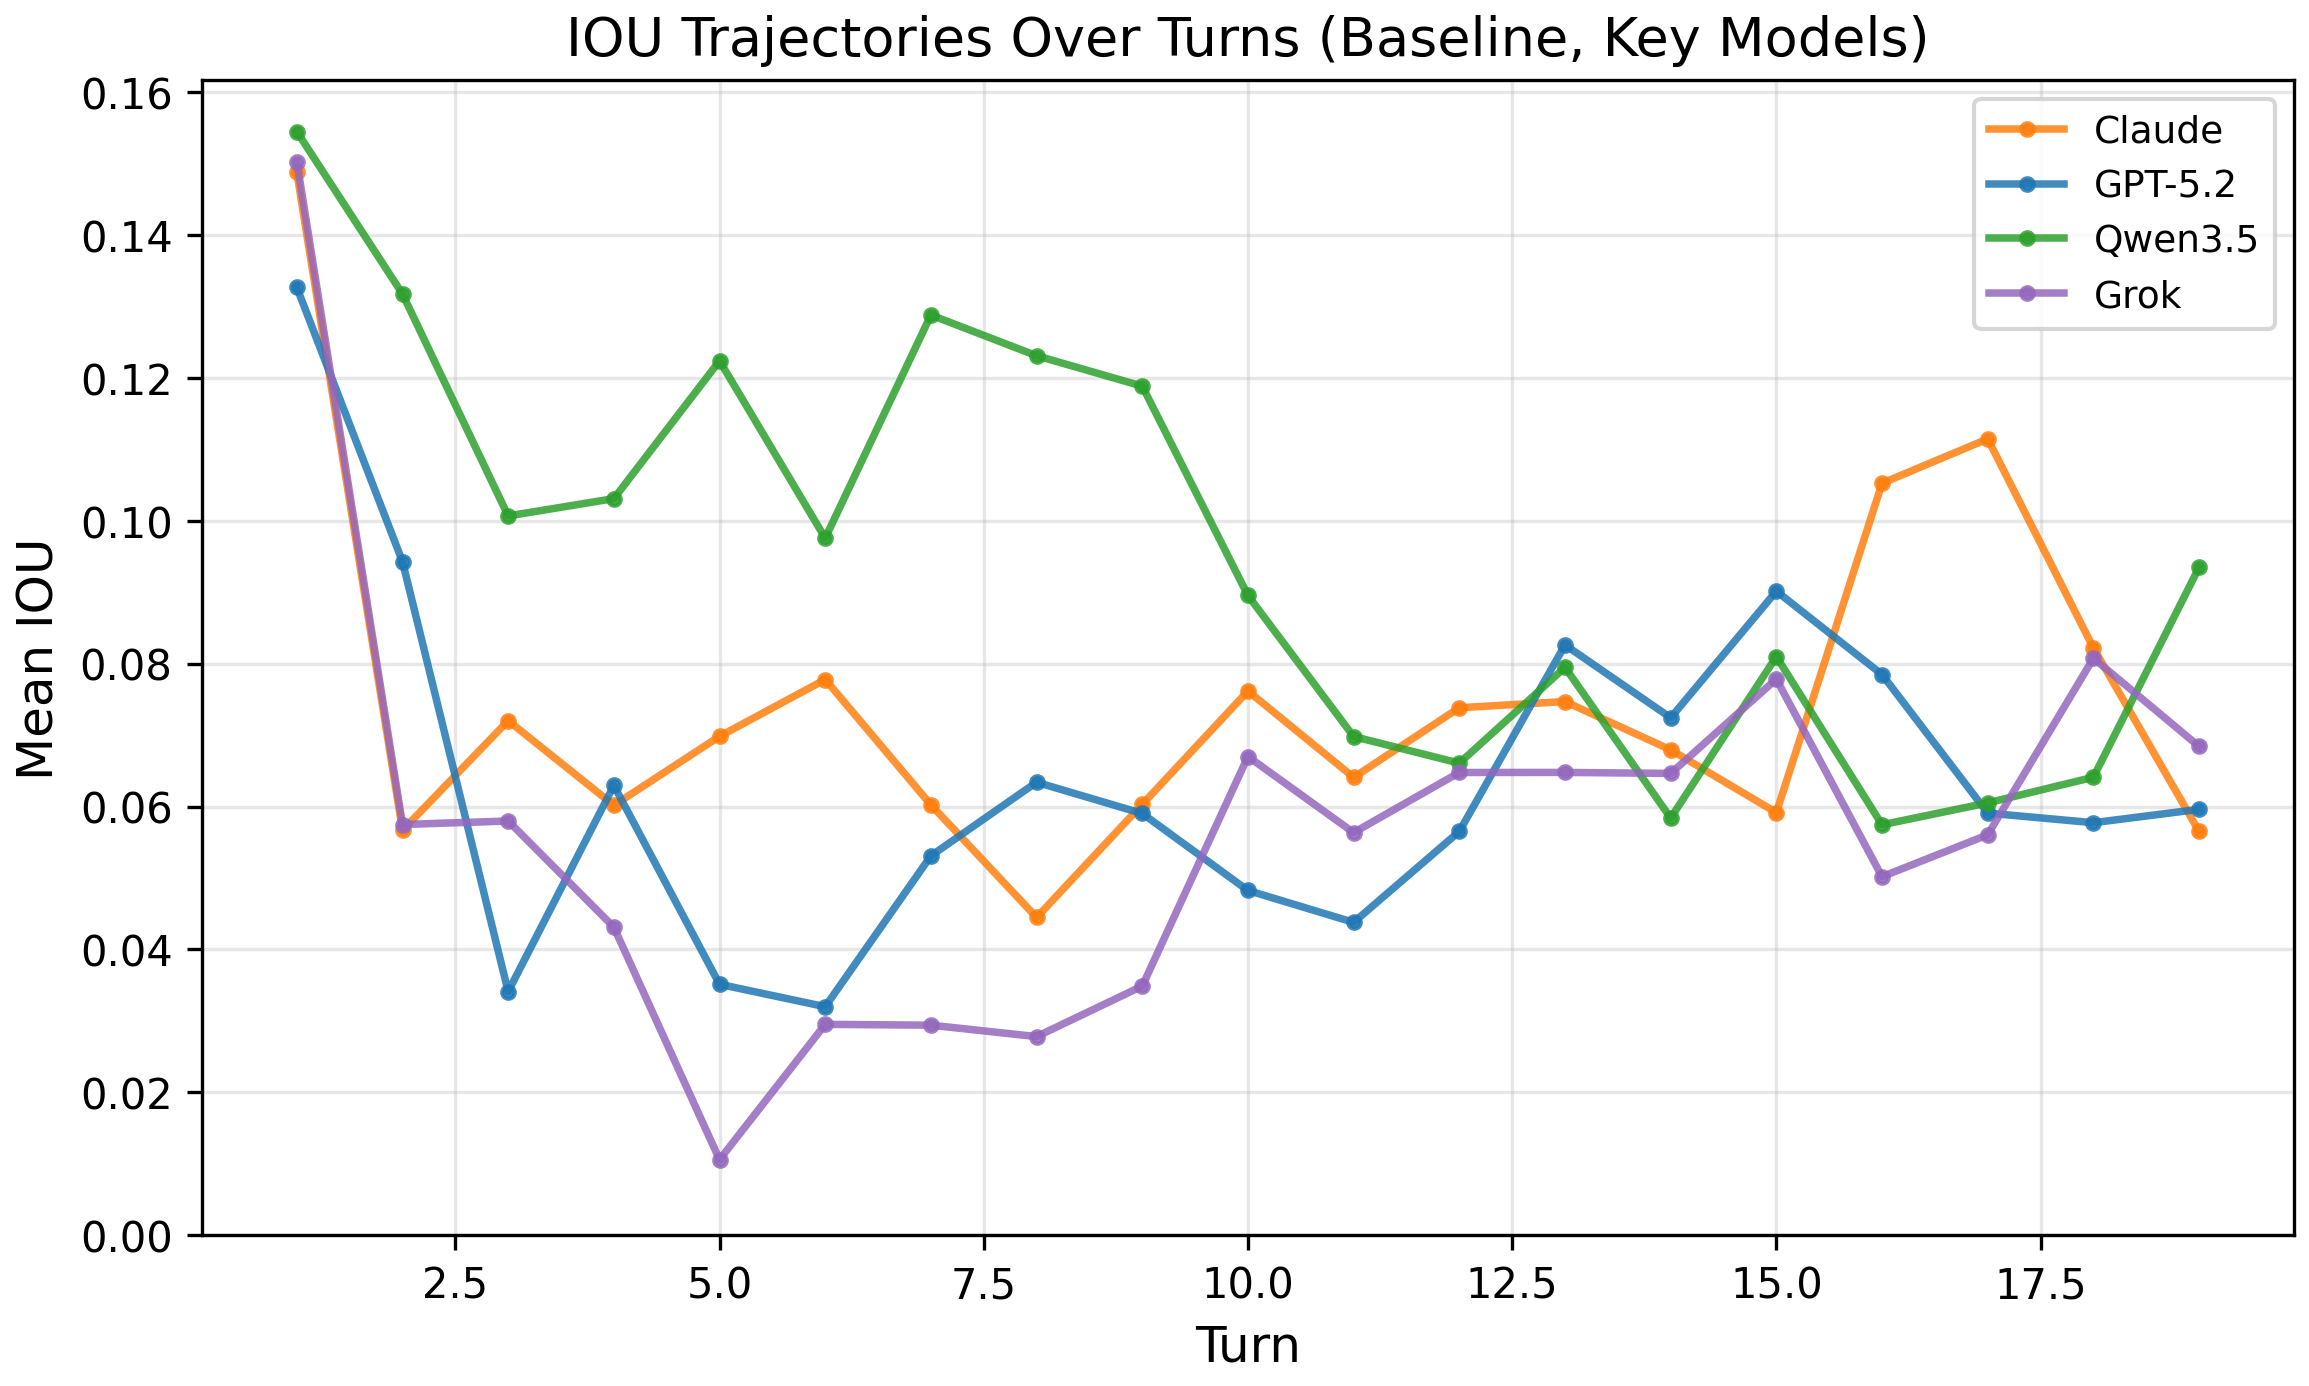
\includegraphics[width=0.8\textwidth]{../experiments_raw_results/wason-2-4-6/figures/wason246_iou_trajectories.png}
    \caption{Траектории среднего IOU по ходам диалога для четырёх ключевых стандартных моделей (baseline, без extended thinking). Все модели демонстрируют высокое начальное IOU с последующим постепенным снижением.}
    \label{fig:246_iou_trajectories}
\end{figure}

\begin{figure}[ht]
    \centering
    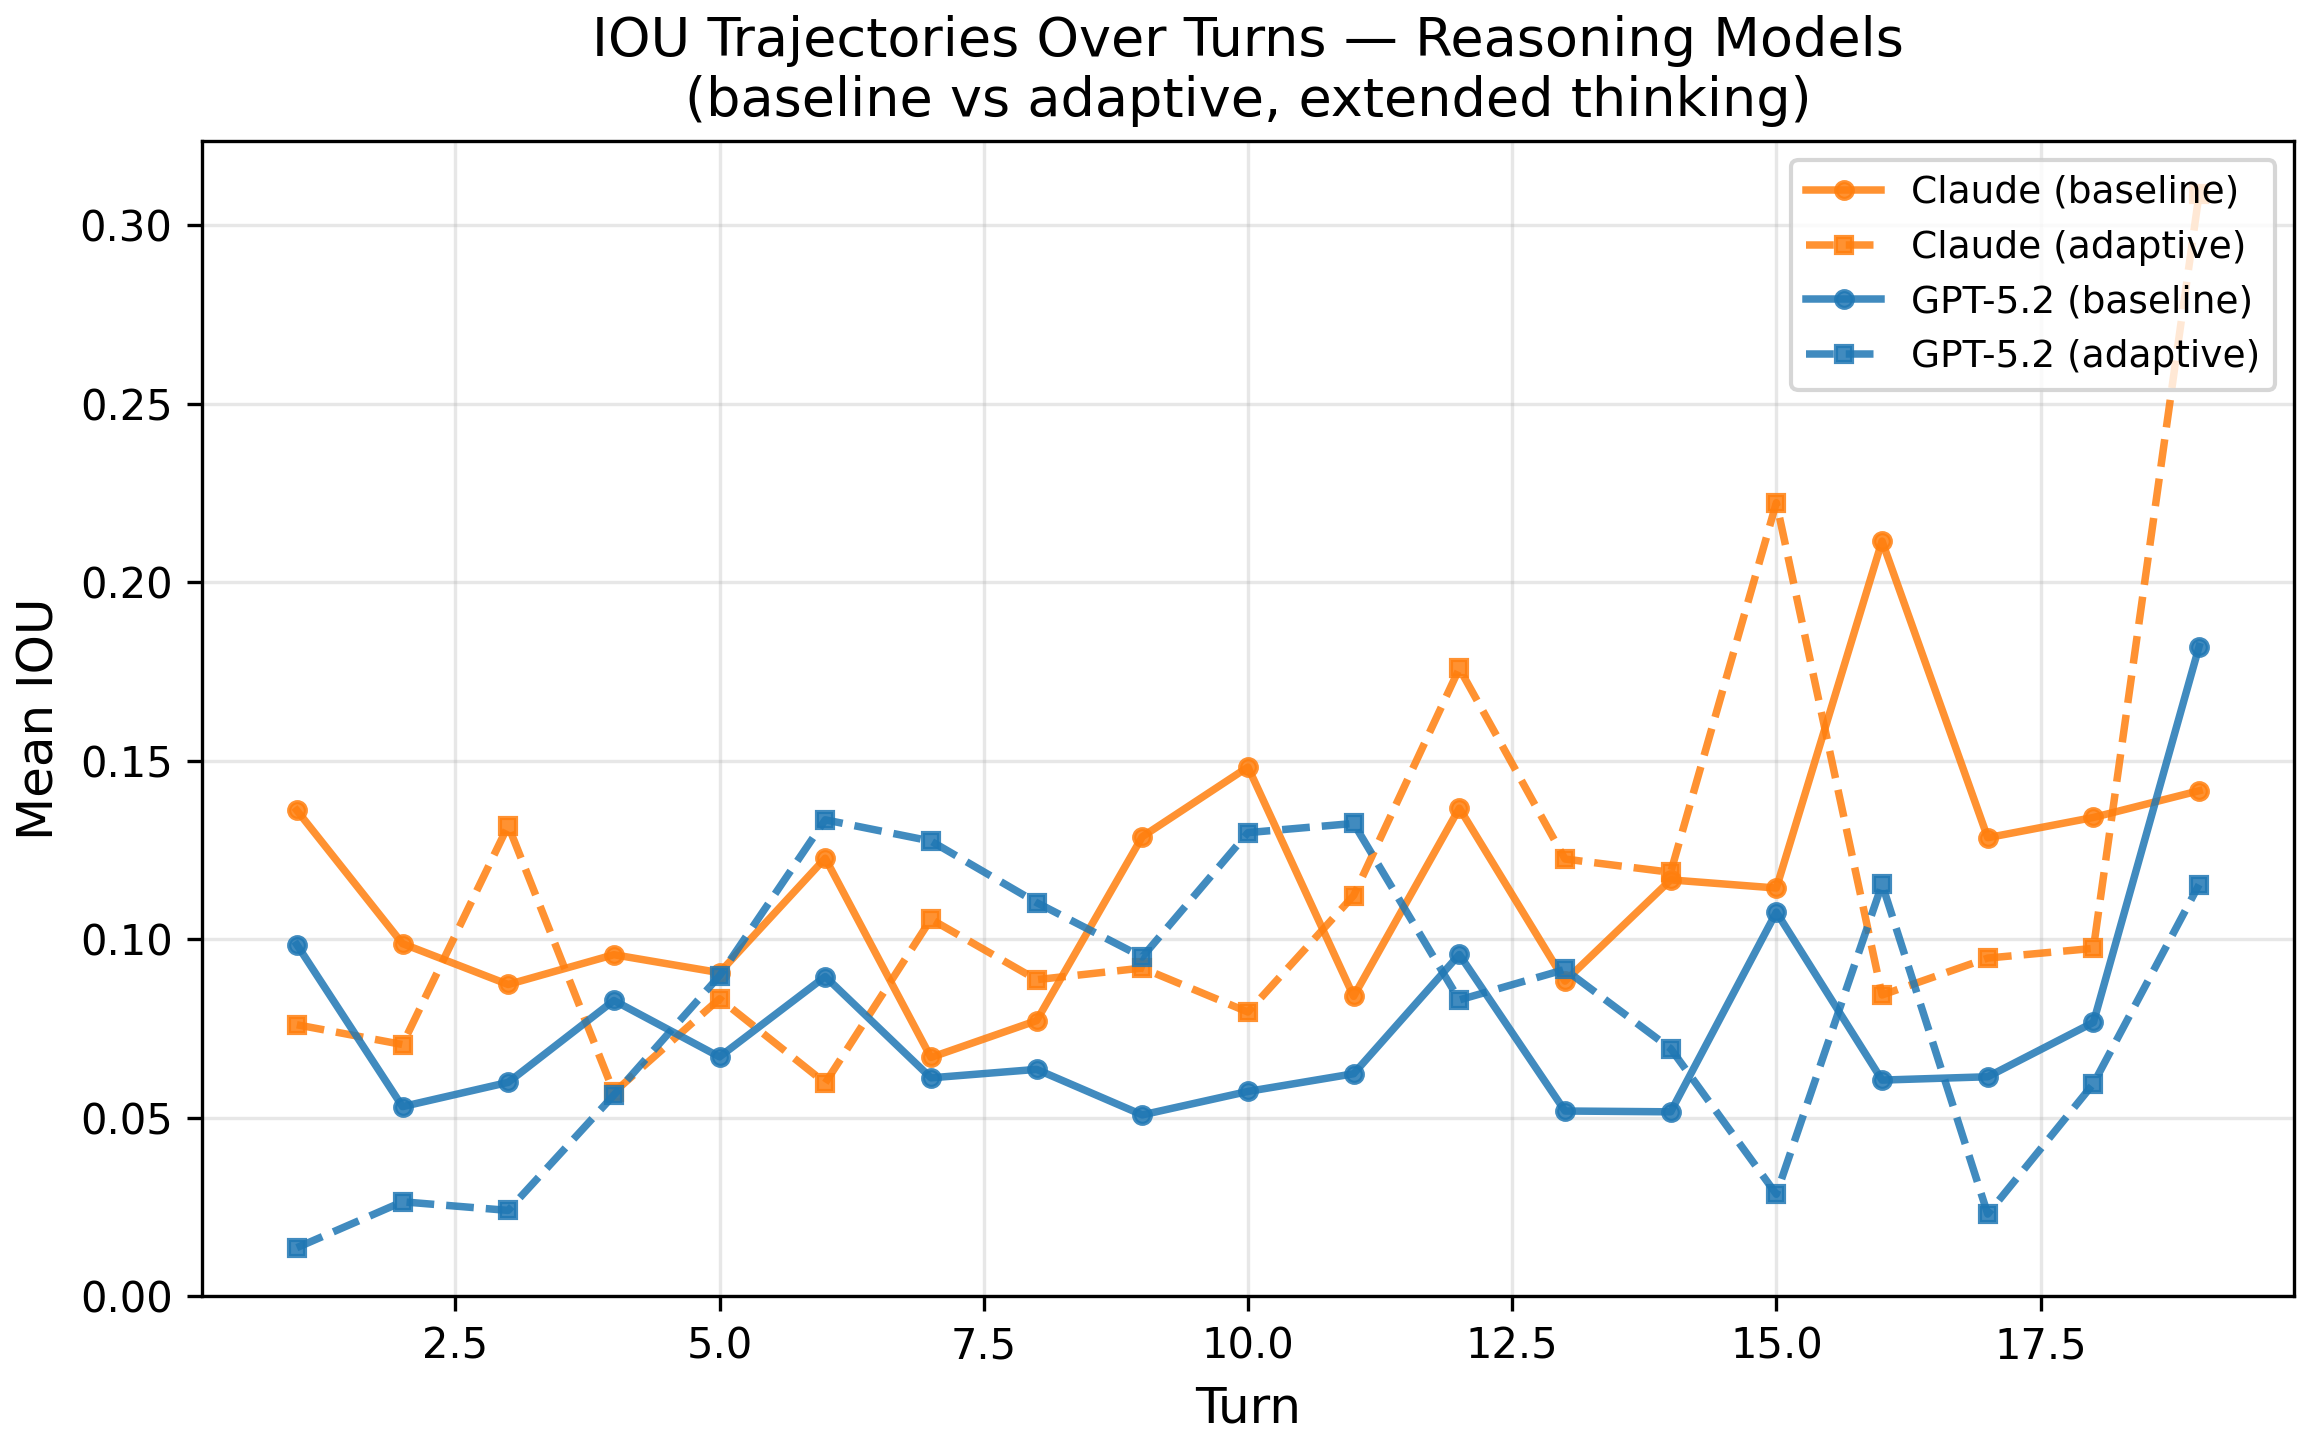
\includegraphics[width=0.8\textwidth]{../experiments_raw_results/wason-2-4-6/figures/wason246_reasoning_iou_trajectories.png}
    \caption{Траектории среднего IOU по ходам диалога для reasoning-моделей (extended thinking). Сплошные линии --- baseline-условие, пунктирные --- adaptive. В отличие от стандартных моделей, IOU у reasoning-моделей не монотонно снижается, а демонстрирует тенденцию к росту на поздних ходах, что свидетельствует о продолжении уточнения гипотезы.}
    \label{fig:246_iou_trajectories_reasoning}
\end{figure}

\textbf{Reasoning даёт качественный скачок.} Как видно на рис.~\ref{fig:246_iou_trajectories}, траектории Reasoning-моделей демонстрируют более быструю и устойчивую сходимость к истинному правилу. \texttt{gpt-5.2} в режиме reasoning (baseline) достигает SR $= 0{,}38$ --- на 10 процентных пунктов выше лучшей non-reasoning модели. В adaptive-условии SR вырастает до 0{,}48 и CTR снижается до 0{,}559, что является единственным случаем CTR ниже 0{,}60 во всём эксперименте. Примечательно, что \texttt{claude-sonnet-4.6 reasoning} также демонстрирует рост SR с 0,28 до 0,32 при адаптивном промпте. Таким образом, reasoning + adaptive --- единственная комбинация, приближающаяся к разумной фальсификационной стратегии, хотя и не достигающая нормативного стандарта.

\textbf{Adaptive-промпт нестабилен.} Из девяти non-reasoning моделей у четырёх SR не изменился или снизился (\texttt{gpt-5.2}: без изменений; \texttt{qwen3.5-397b-a17b}: $0{,}22 \to 0{,}18$; \texttt{grok-4.1-fast}: $0{,}14 \to 0{,}08$; \texttt{gemma-3-12b-it}: $0{,}06 \to 0{,}04$). Снижение CTR не гарантирует роста SR. На рис.~\ref{fig:246_scatter_sr_correlation} показана корреляция между стратегией тестирования (CTR) и итоговым успехом (SR) --- заметно, что снижение CTR помогает reasoning-моделям, но слабо влияет на эффективность большинства non-reasoning моделей.

\begin{figure}[ht]
    \centering
    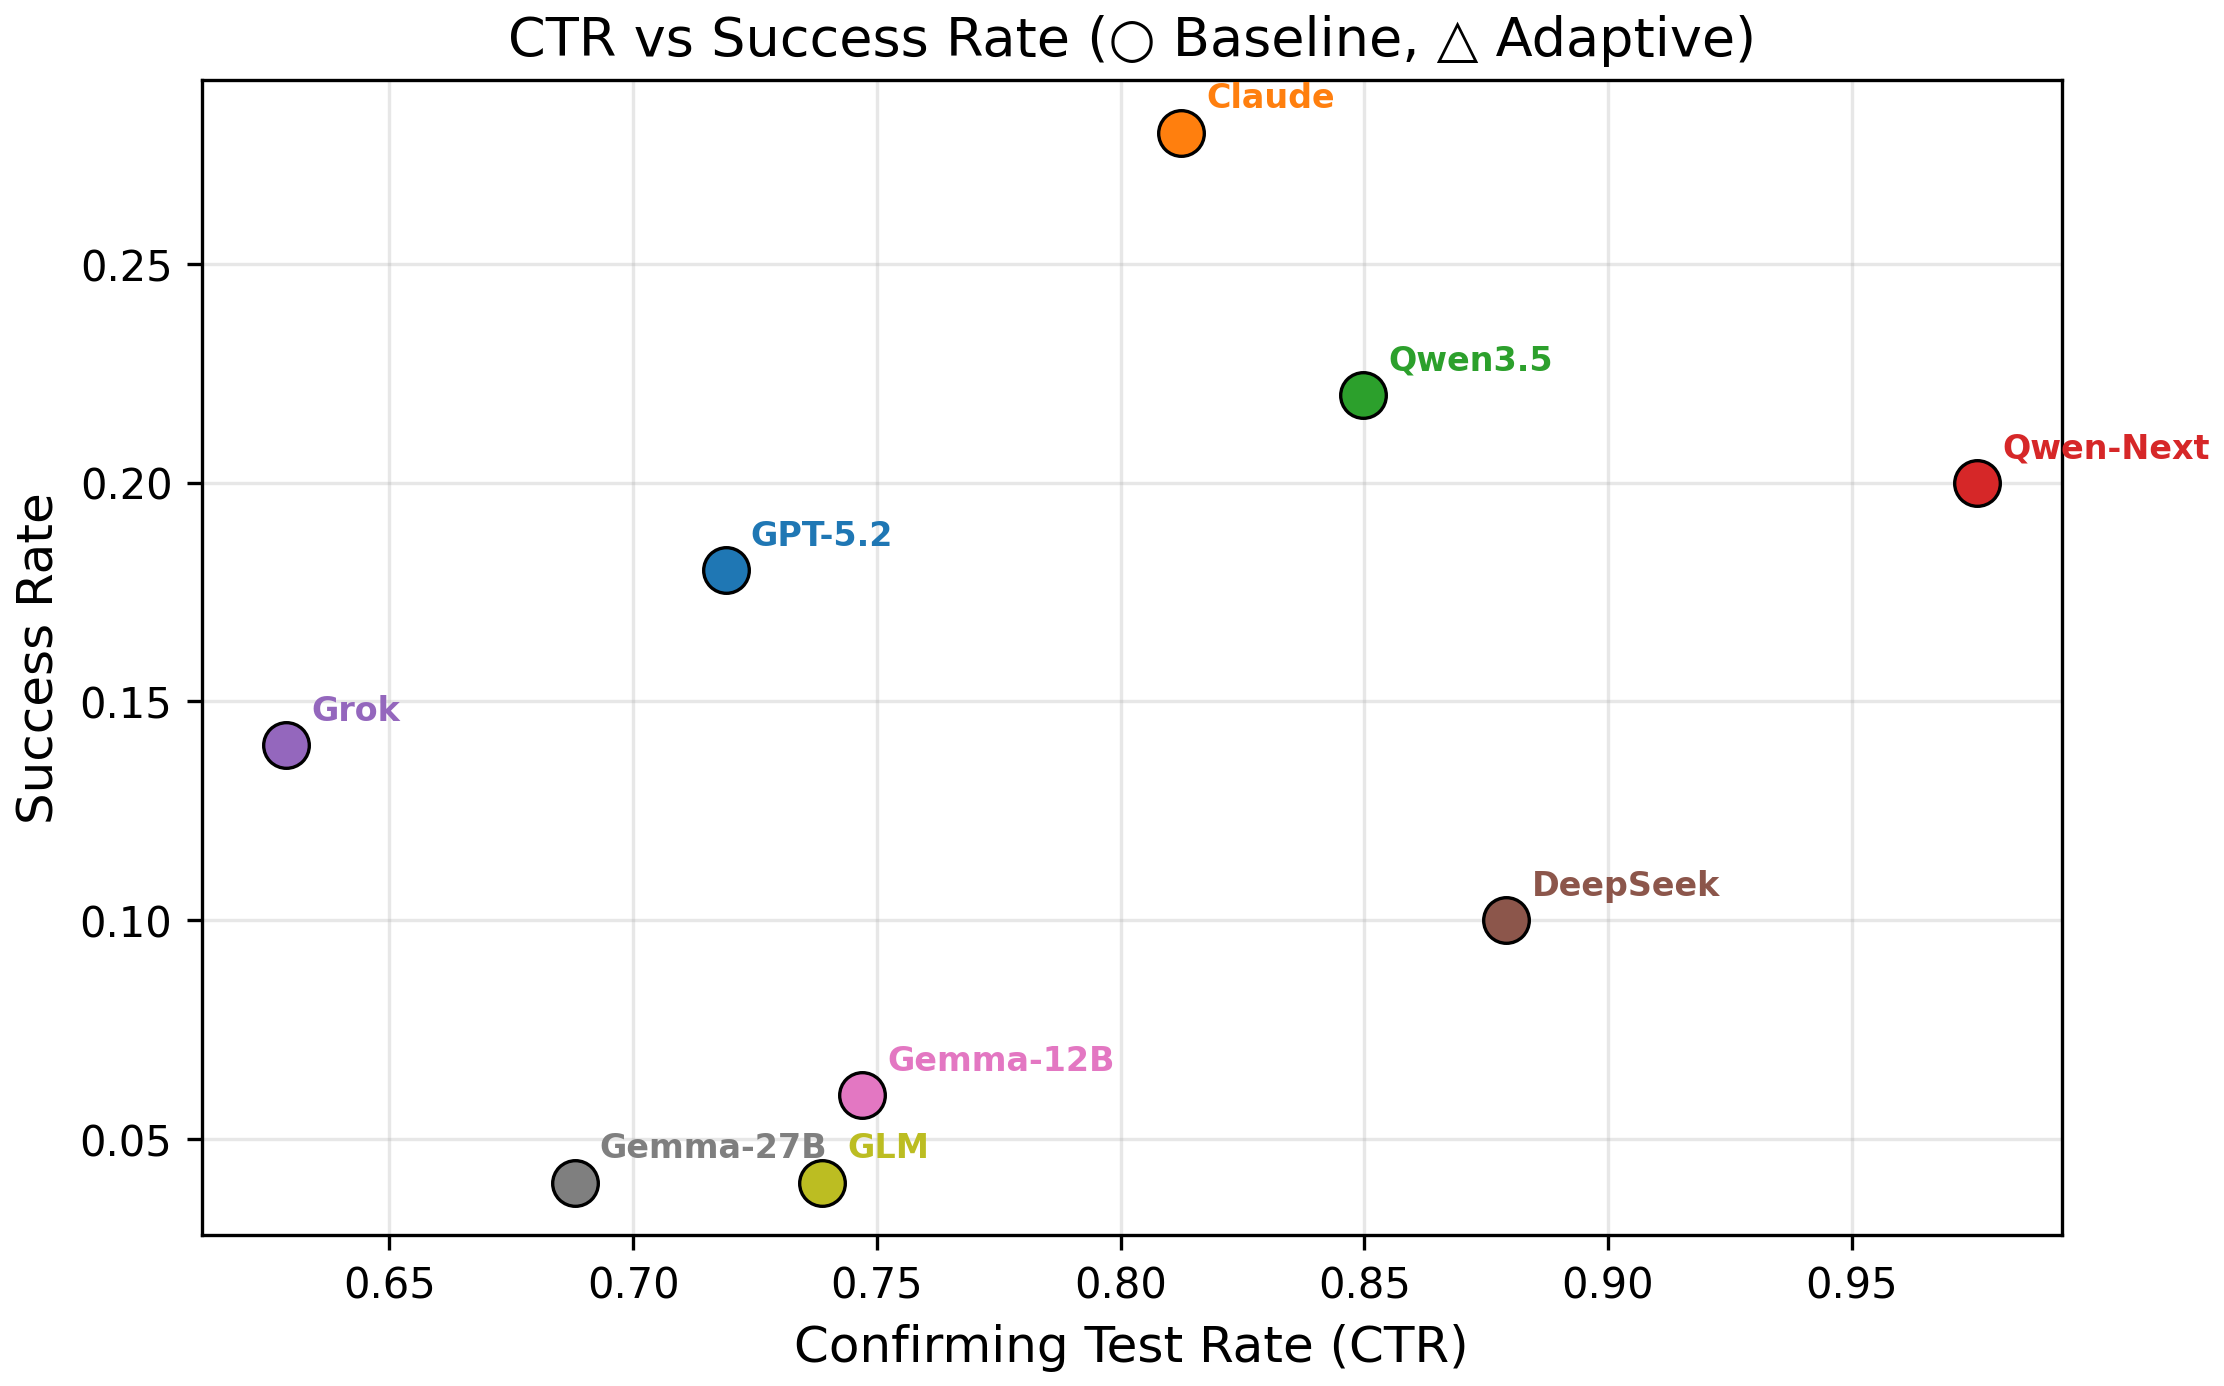
\includegraphics[width=0.8\textwidth]{../experiments_raw_results/wason-2-4-6/figures/wason246_scatter_sr_correlation.png}
    \caption{Корреляция между CTR и Success Rate. Пунктирная линия разделяет reasoning и non-reasoning модели.}
    \label{fig:246_scatter_sr_correlation}
\end{figure}

Наиболее интригующим является \textbf{парадокс \texttt{qwen3.5-397b-a17b}}: adaptive-промпт вызвал крупнейшее снижение CTR среди non-reasoning моделей ($0{,}850 \to 0{,}602$, то есть модель стала значительно активнее фальсифицировать), однако SR упал с 0{,}22 до 0{,}18. Модель начала тестировать опровергающие тройки, но не смогла конвертировать это в правильную гипотезу --- что указывает на разрыв между стратегией тестирования и качеством обновления гипотез.

\begin{figure}[ht]
    \centering
    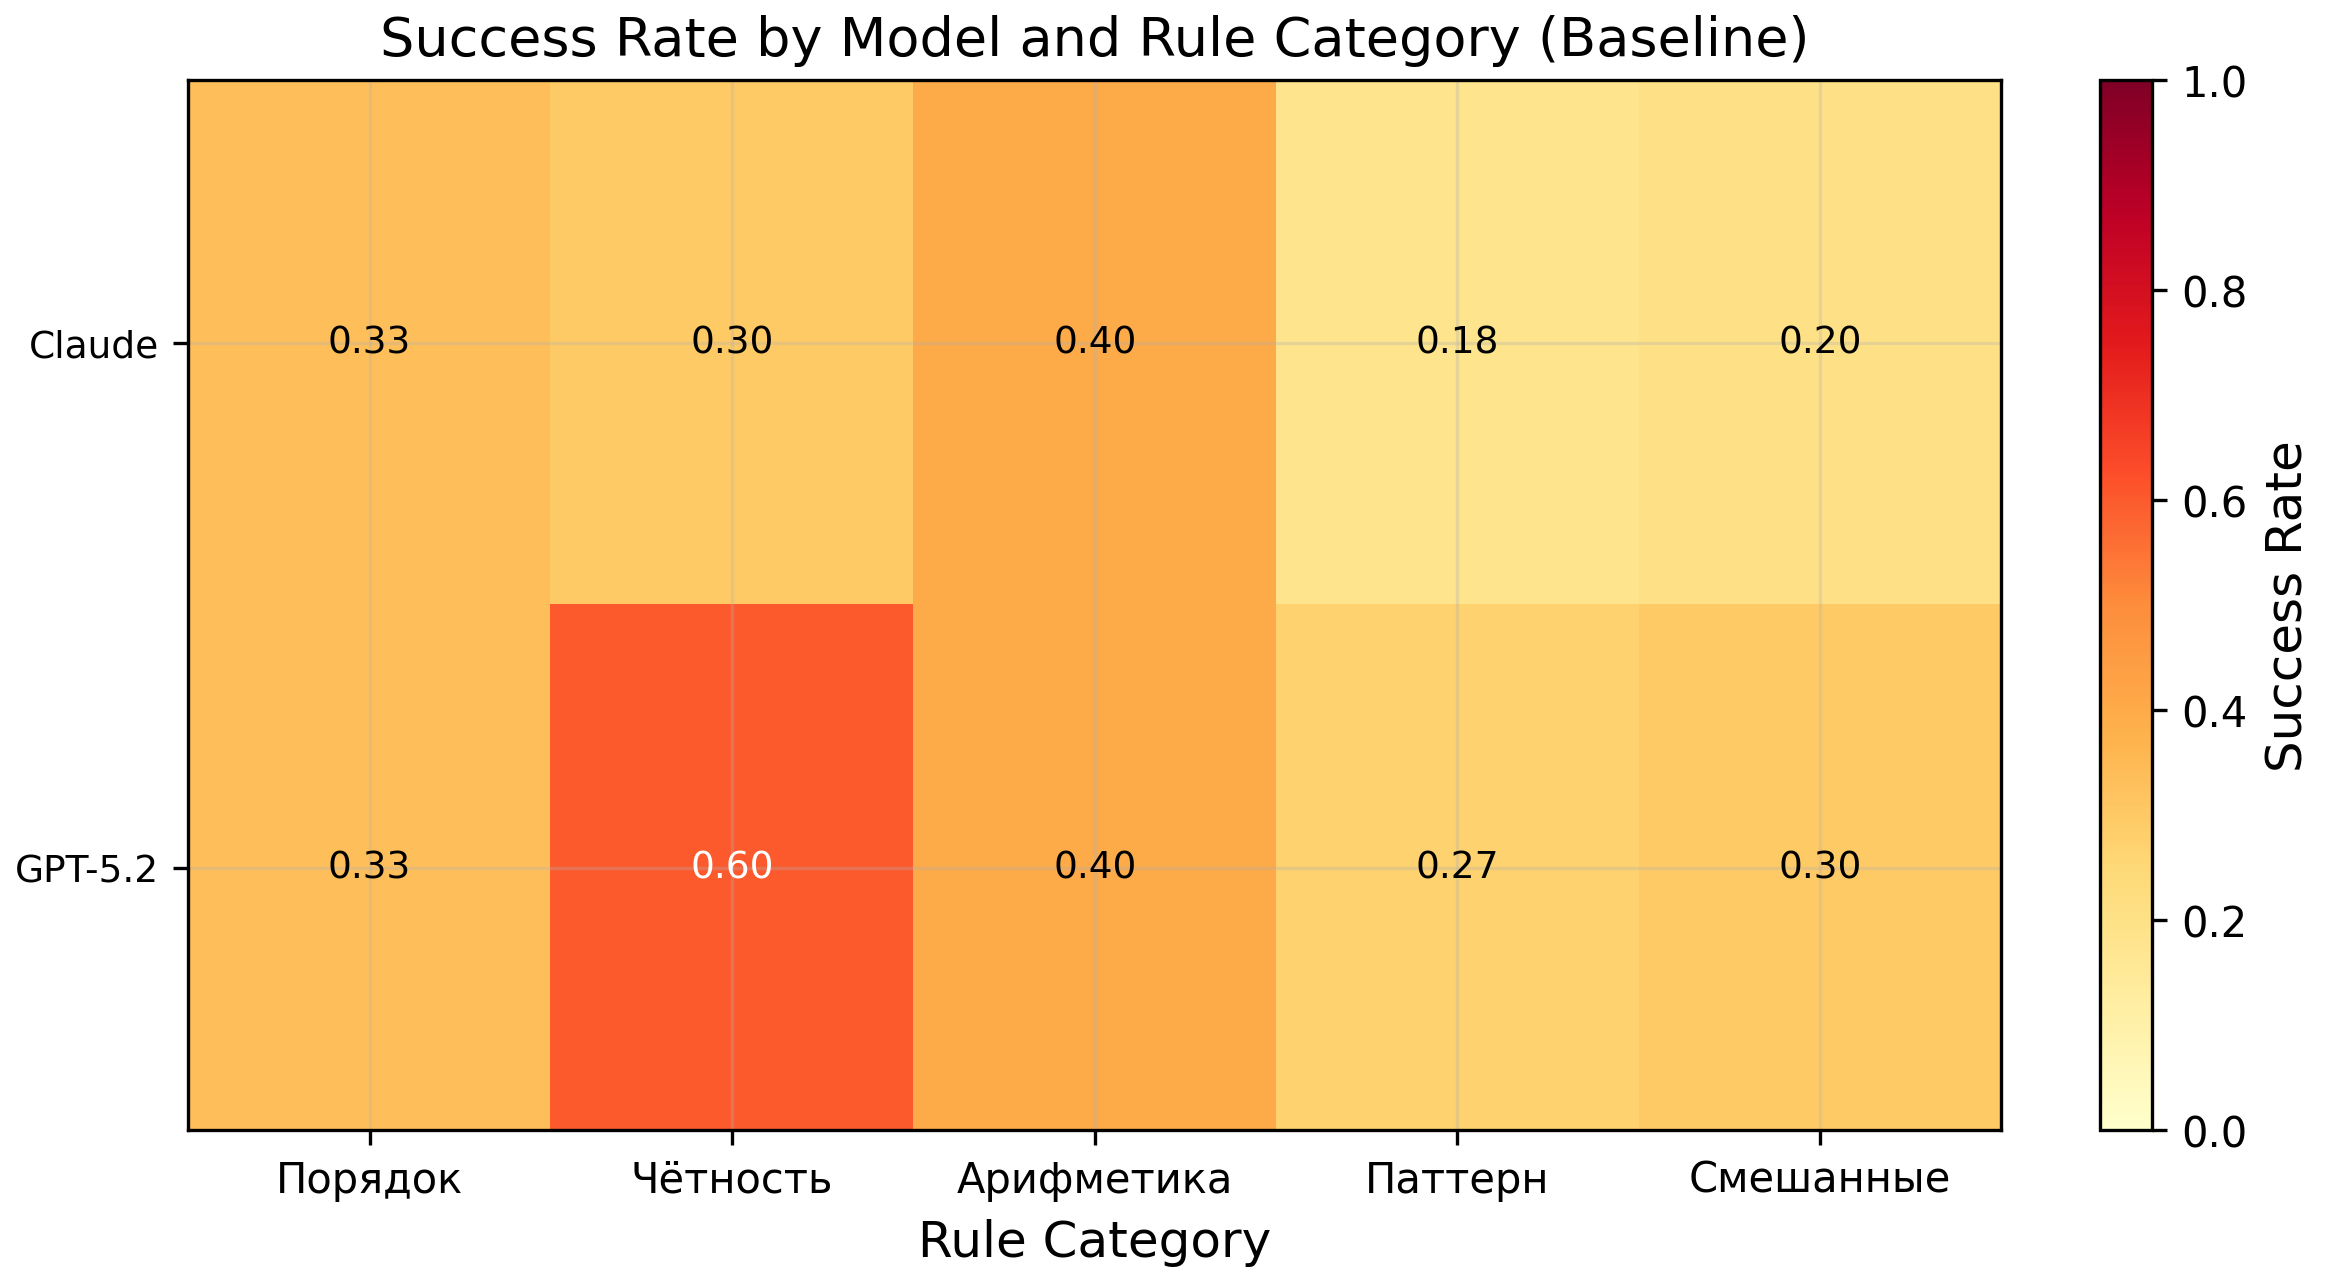
\includegraphics[width=0.9\textwidth]{../experiments_raw_results/wason-2-4-6/figures/wason246_category_heatmap.png}
    \caption{Тепловая карта Success Rate по категориям правил. Наибольшую сложность представляют структурные паттерны и смешанные правила.}
    \label{fig:246_category_heatmap}
\end{figure}

\textbf{Контринтуитивный эффект у \texttt{gemma-3-27b-it}:} adaptive-промпт, направленный на фальсификацию, \textit{увеличил} CTR ($0{,}688 \to 0{,}842$), однако SR при этом вырос с 0{,}04 до 0{,}10. Это указывает на то, что данная модель находит правильную гипотезу не через фальсифицирующую стратегию, а через какой-то иной механизм, нечувствительный к инструкциям по типу тестов. Анализ по категориям (рис.~\ref{fig:246_category_heatmap}) показывает, что категория «Структурные паттерны» (например, «ровно два уникальных значения») является наиболее труднодоступной для моделей, в то время как правила на порядок и сравнение («строго возрастающая последовательность») обнаруживаются значительно чаще.

\textbf{AUC-IOU} выявляет расхождение между качеством траектории и финальным результатом. У \texttt{gpt-5.2} reasoning при переходе baseline $\to$ adaptive: SR $+0{,}10$, но AUC-IOU $0{,}119 \to 0{,}082$ --- менее гладкая траектория сходимости при лучшем финальном результате. У \texttt{deepseek-v3.2} в baseline AUC-IOU ($0{,}052$) существенно ниже, чем у \texttt{claude-sonnet-4.6} ($0{,}127$), при схожем SR, что указывает на «спринт» к правильному ответу в последних ходах без устойчивого накопления качества гипотезы.

\begin{figure}[ht]
    \centering
    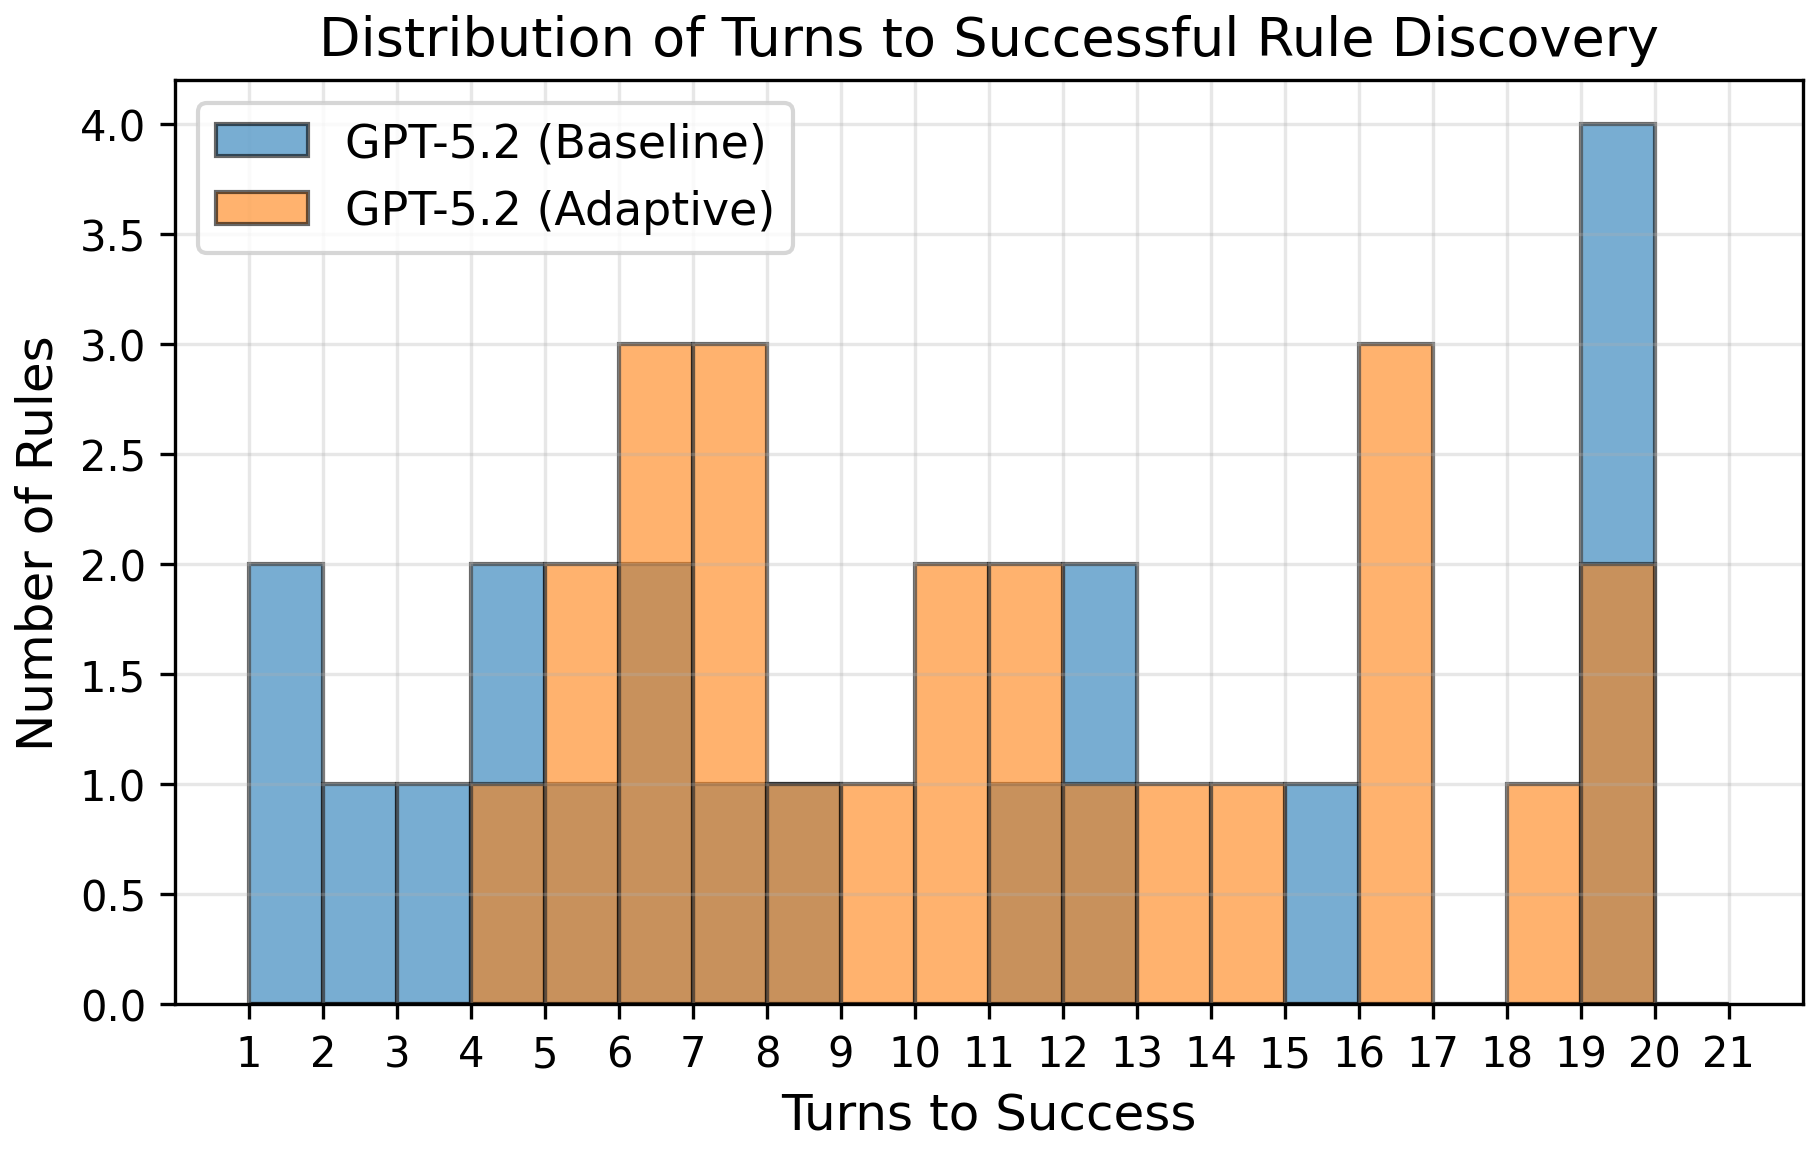
\includegraphics[width=0.7\textwidth]{../experiments_raw_results/wason-2-4-6/figures/wason246_turns_to_success.png}
    \caption{Среднее количество ходов до успешного обнаружения правила. Reasoning-модели приходят к решению существенно быстрее.}
    \label{fig:246_turns_to_success}
\end{figure}

\textbf{Hypothesis Change Rate (HCR)} в baseline варьируется от 0,622 у \texttt{gpt-5.2} до 0,940 у \texttt{gemma-3-27b-it}. Adaptive-промпт влияет на HCR неоднородно: у \texttt{deepseek-v3.2} HCR снижается с 0,833 до 0,595 (модель реже меняет гипотезу), у \texttt{gemma-3-27b-it} --- с 0,940 до 0,892, у \texttt{glm-4.7-flash} --- с 0,649 до 0,543. У ряда моделей (\texttt{qwen3.5-397b-a17b}: $0{,}654 \to 0{,}750$; \texttt{qwen3-next-80b}: $0{,}665 \to 0{,}732$) HCR при adaptive растёт --- модели активнее пересматривают гипотезы. Таким образом, adaptive-промпт влияет на поведение ревизии гипотез, однако это влияние не транслируется напрямую в рост SR. Как видно на рис.~\ref{fig:246_turns_to_success}, те модели, которые все же находят правило, в режиме Adaptive делают это за меньшее количество ходов.

\subsection{Выводы по эксперименту 3}

Эксперимент 3 установил: (1)~предубеждение подтверждения в индуктивном рассуждении универсально --- CTR $\geq 0{,}629$ у всех non-reasoning моделей в baseline; (2)~reasoning даёт качественный скачок, недостижимый через prompt engineering: SR \texttt{gpt-5.2} reasoning = 0{,}48 против максимума 0{,}28 у non-reasoning; (3)~adaptive-промпт нестабилен: снижение CTR не конвертируется в рост SR у половины моделей; (4)~парадокс \texttt{qwen3.5-397b-a17b} --- разрыв между стратегией тестирования и качеством обновления гипотез --- указывает на то, что предубеждение подтверждения имеет как минимум два независимых компонента: выбор тестируемых троек и ревизию гипотез.
